\documentclass[aspectratio=169]{beamer}

\mode<presentation>
{
  \usetheme{default}
  \usecolortheme{default}
  \usefonttheme{default}
  \setbeamertemplate{navigation symbols}{}
  \setbeamertemplate{caption}[numbered]
  \setbeamertemplate{footline}[frame number]  % or "page number"
  \setbeamercolor{frametitle}{fg=white}
  \setbeamercolor{footline}{fg=black}
} 

\usepackage[english]{babel}
\usepackage[utf8x]{inputenc}
\usepackage{tikz}
\usepackage{courier}
\usepackage{array}
\usepackage{bold-extra}
\usepackage{minted}
\usepackage[thicklines]{cancel}
\usepackage{fancyvrb}

\xdefinecolor{dianablue}{rgb}{0.18,0.24,0.31}
\xdefinecolor{darkblue}{rgb}{0.1,0.1,0.7}
\xdefinecolor{darkgreen}{rgb}{0,0.5,0}
\xdefinecolor{darkgrey}{rgb}{0.35,0.35,0.35}
\xdefinecolor{darkorange}{rgb}{0.8,0.5,0}
\xdefinecolor{darkred}{rgb}{0.7,0,0}
\definecolor{darkgreen}{rgb}{0,0.6,0}
\definecolor{mauve}{rgb}{0.58,0,0.82}

\definecolor{mycolor}{HTML}{FF6600}
\definecolor{cppcolor}{HTML}{00AAD4}
\definecolor{rootcolor}{HTML}{2A2AFF}
\definecolor{rootnpcolor}{HTML}{008000}
\definecolor{pythoncolor}{HTML}{FF00CC}

\title[2018-07-10-chep-columnar]{Columnar data processing for HEP analysis}
\author{Jim Pivarski}
\institute{Princeton University -- DIANA-HEP}
\date{July 10, 2018}

\begin{document}

\logo{\pgfputat{\pgfxy(0.11, 7.4)}{\pgfbox[right,base]{\tikz{\filldraw[fill=dianablue, draw=none] (0 cm, 0 cm) rectangle (50 cm, 1 cm);}\mbox{\hspace{-8 cm}
\includegraphics[height=1 cm]{princeton-logo-long.png}
\includegraphics[height=1 cm]{diana-hep-logo-long.png}}}}}

\begin{frame}
  \titlepage
\end{frame}

\logo{\pgfputat{\pgfxy(0.11, 7.4)}{\pgfbox[right,base]{\tikz{\filldraw[fill=dianablue, draw=none] (0 cm, 0 cm) rectangle (50 cm, 1 cm);}\mbox{\hspace{-8 cm}
\includegraphics[height=1 cm]{princeton-logo.png}
\includegraphics[height=1 cm]{diana-hep-logo.png}}}}}

% Uncomment these lines for an automatically generated outline.
%\begin{frame}{Outline}
%  \tableofcontents
%\end{frame}

% START START START START START START START START START START START START START

\begin{frame}{Motivation}
\vspace{0.5 cm}
\large
In the late stages of data analysis, only order-of-magnitude speedups translate into human productivity, and only if they're easy to set up.

\vspace{0.5 cm}
\uncover<2->{Producing a plot in a second instead of an hour is life-changing, but not if it takes two hours to write the script.}
\end{frame}

\begin{frame}{Motivation}
\begin{columns}
\column{0.41\linewidth}
However, most HEP analysis doesn't optimize for the most critical performance bottleneck: data layout in memory.

\vspace{0.5 cm}
Modern processors are much faster than memory, so arranging data for dense, sequential scanning is critical. \textcolor{gray}{(a.k.a.\ ``struct of arrays'')}

\vspace{0.5 cm}
However, it can be hard to set up and analyze data in this form.
\column{0.55\linewidth}
\vspace{0.3 cm}
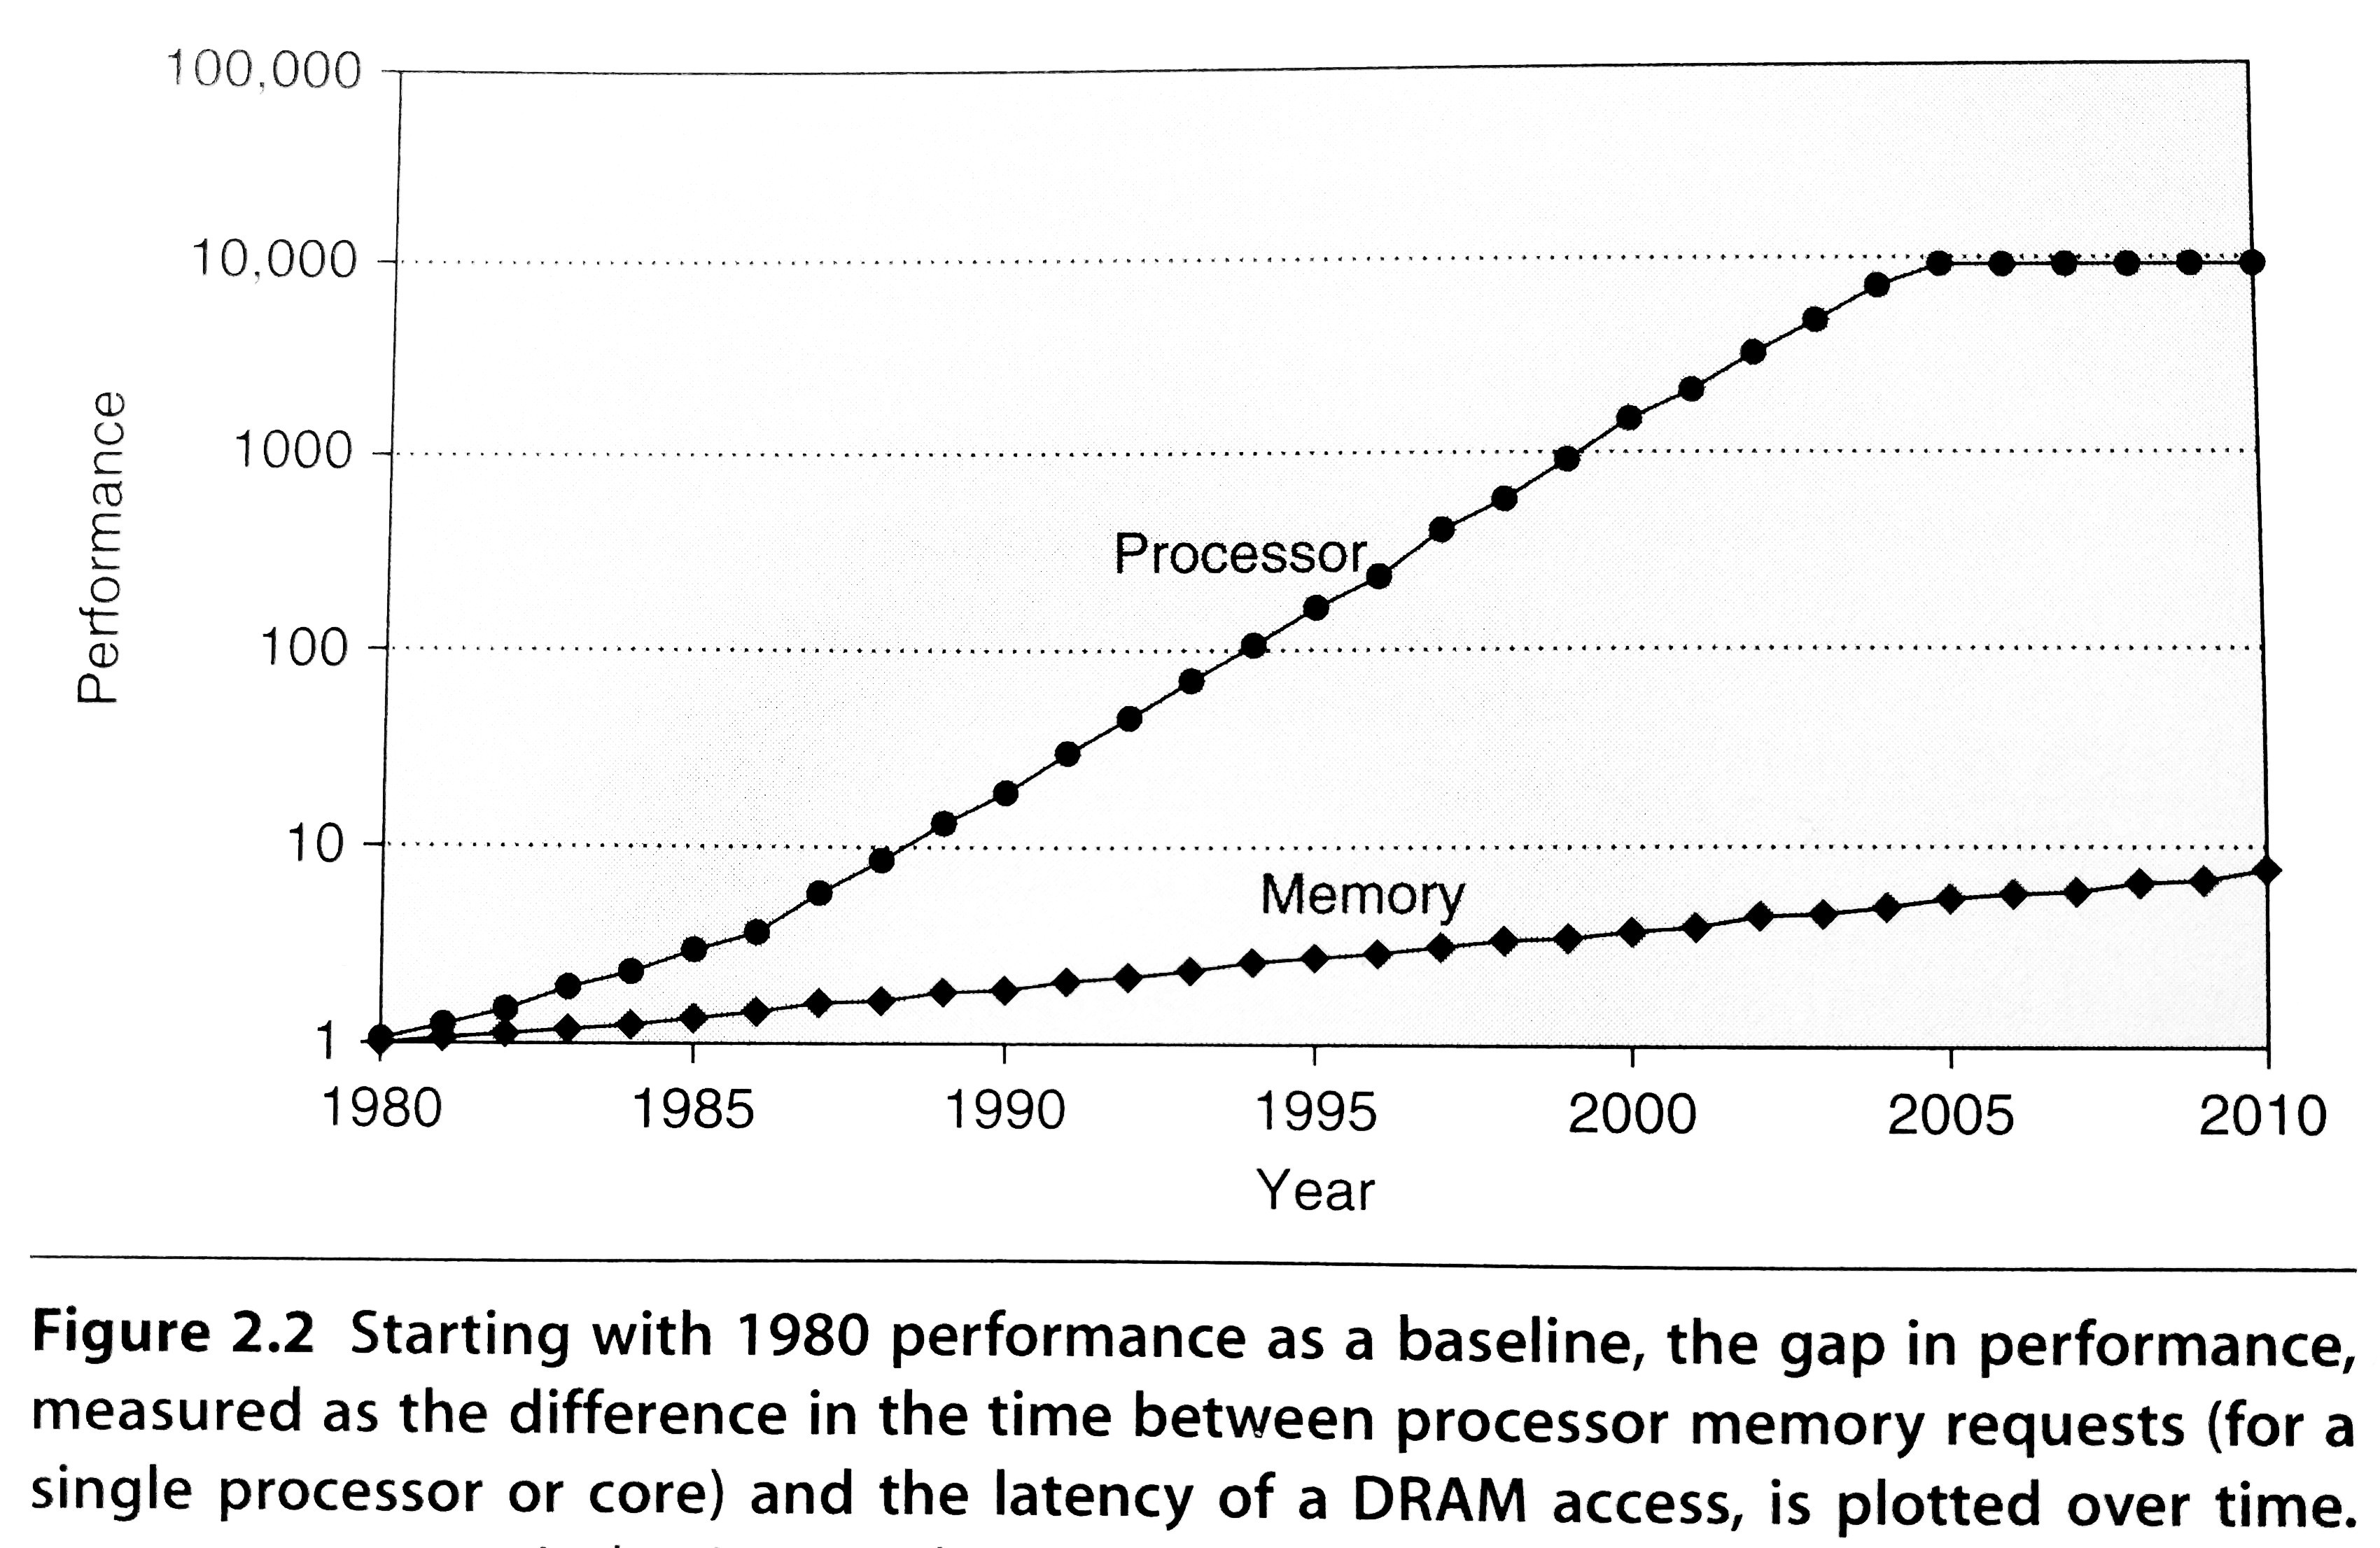
\includegraphics[width=\linewidth]{performance-gap.jpg}

\vspace{0.25 cm}
\begin{columns}
\column{0.2\linewidth}
\column{0.4\linewidth}
\tiny
From Hennessy \& Patterson, {\it Computer Architecture, A~Quantitative Approach.}

\column{0.25\linewidth}
\hspace{-0.5 cm}
\includegraphics[width=\linewidth]{hennessy-book.jpg}
\end{columns}
\end{columns}
\end{frame}

\begin{frame}[fragile]{Motivation}
\vspace{0.2 cm}
Columnar data representations get particularly complex for hierarchically nested data.

\vspace{0.25 cm}
\begin{columns}
\column{0.2\linewidth}
\column{0.3\linewidth}
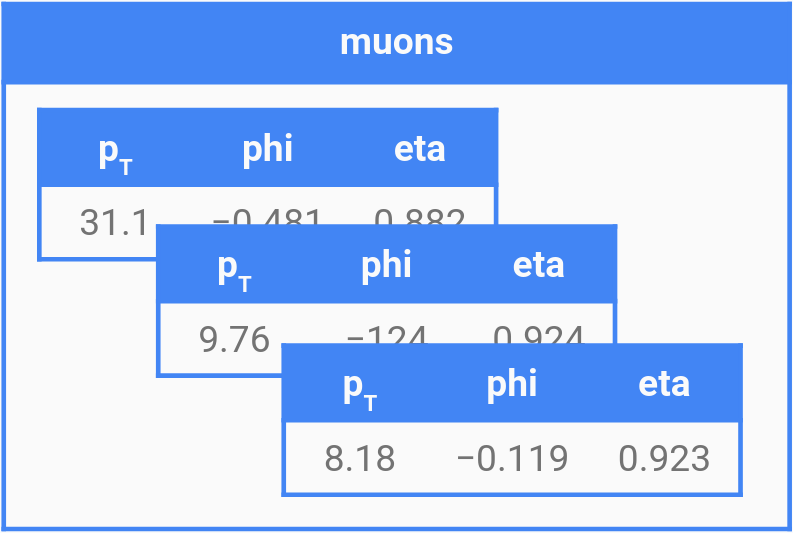
\includegraphics[width=\linewidth]{muons-as-objects.png}

\column{0.05\linewidth}
\centering vs

\column{0.3\linewidth}
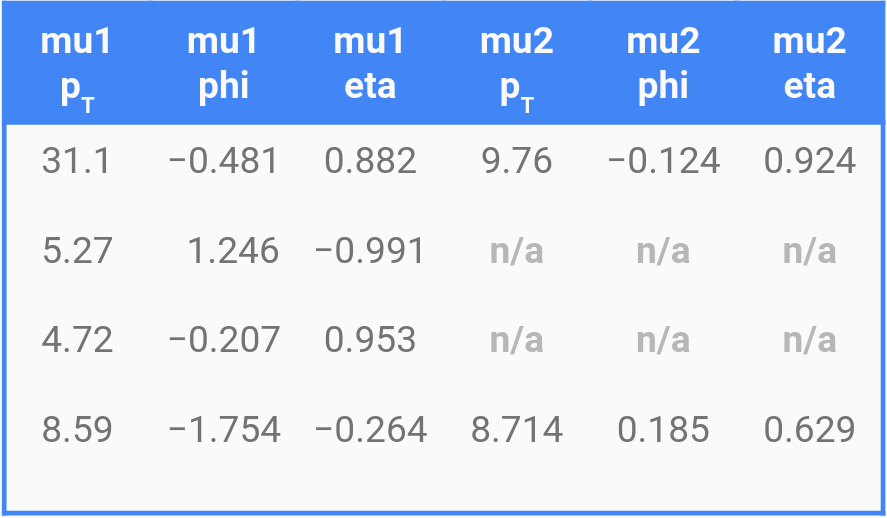
\includegraphics[width=\linewidth]{muons-as-a-table.png}
\column{0.2\linewidth}
\end{columns}

\vspace{0.25 cm}
\scriptsize
\begin{Verbatim}[commandchars=\\\{\}]
[[Muon(\textcolor{darkgreen}{31.1}, \textcolor{darkorange}{-0.481}, \textcolor{blue}{0.882}), Muon(\textcolor{darkgreen}{9.76}, \textcolor{darkorange}{-0.124}, \textcolor{blue}{0.924}), Muon(\textcolor{darkgreen}{8.18}, \textcolor{darkorange}{-0.119}, \textcolor{blue}{0.923})],
 [Muon(\textcolor{darkgreen}{5.27}, \textcolor{darkorange}{1.246}, \textcolor{blue}{-0.991})],
 [Muon(\textcolor{darkgreen}{4.72}, \textcolor{darkorange}{-0.207}, \textcolor{blue}{0.953})],
 [Muon(\textcolor{darkgreen}{8.59}, \textcolor{darkorange}{-1.754}, \textcolor{blue}{-0.264}), Muon(\textcolor{darkgreen}{8.714}, \textcolor{darkorange}{0.185}, \textcolor{blue}{0.629})],
 ...
\end{Verbatim}

{\normalsize becomes four contiguous arrays:}

\vspace{0.25 cm}
\begin{tabular}{r l}
\small offsets &                    {\tt\scriptsize \ \ \ \ \ 0,\ \ \ \ \ \ \ \ \ \ \ \ \ \ \ \ \ \ \ \ \ \ 3,\ \ \ \ \ \ 4,\ \ \ \ \ \ 5,\ \ \ \ \ \ \ 7} \\
\small $p_T$ & \textcolor{darkgreen}{\tt\scriptsize \ \ 31.1,\ \ \ 9.76,\ \ \ 8.18,\ \ \ 5.27,\ \ \ 4.72,\ \ \ 8.59, 8.714} \\
\small phi &  \textcolor{darkorange}{\tt\scriptsize -0.481,\ -0.123,\ -0.119,\ \ 1.246,\ -0.207,\ -1.754,\ 0.185} \\
\small eta &        \textcolor{blue}{\tt\scriptsize \ 0.882,\ \ 0.924,\ \ 0.923,\ -0.991,\ \ 0.953,\ -0.264,\ 0.629} \\
\end{tabular}
\end{frame}

\begin{frame}{This talk will be about:}
\vspace{0.5 cm}
\Large
\begin{center}
\textcolor{darkblue}{Vertical performance through columnar data}

\vspace{0.5 cm}
{\it and}

\vspace{0.5 cm}
\textcolor{darkblue}{Convenient syntax for analysis scripts}
\end{center}
\end{frame}

\begin{frame}{Landscape of vertical performance}
\vspace{0.3 cm}
\begin{columns}
\column{1.15\linewidth}
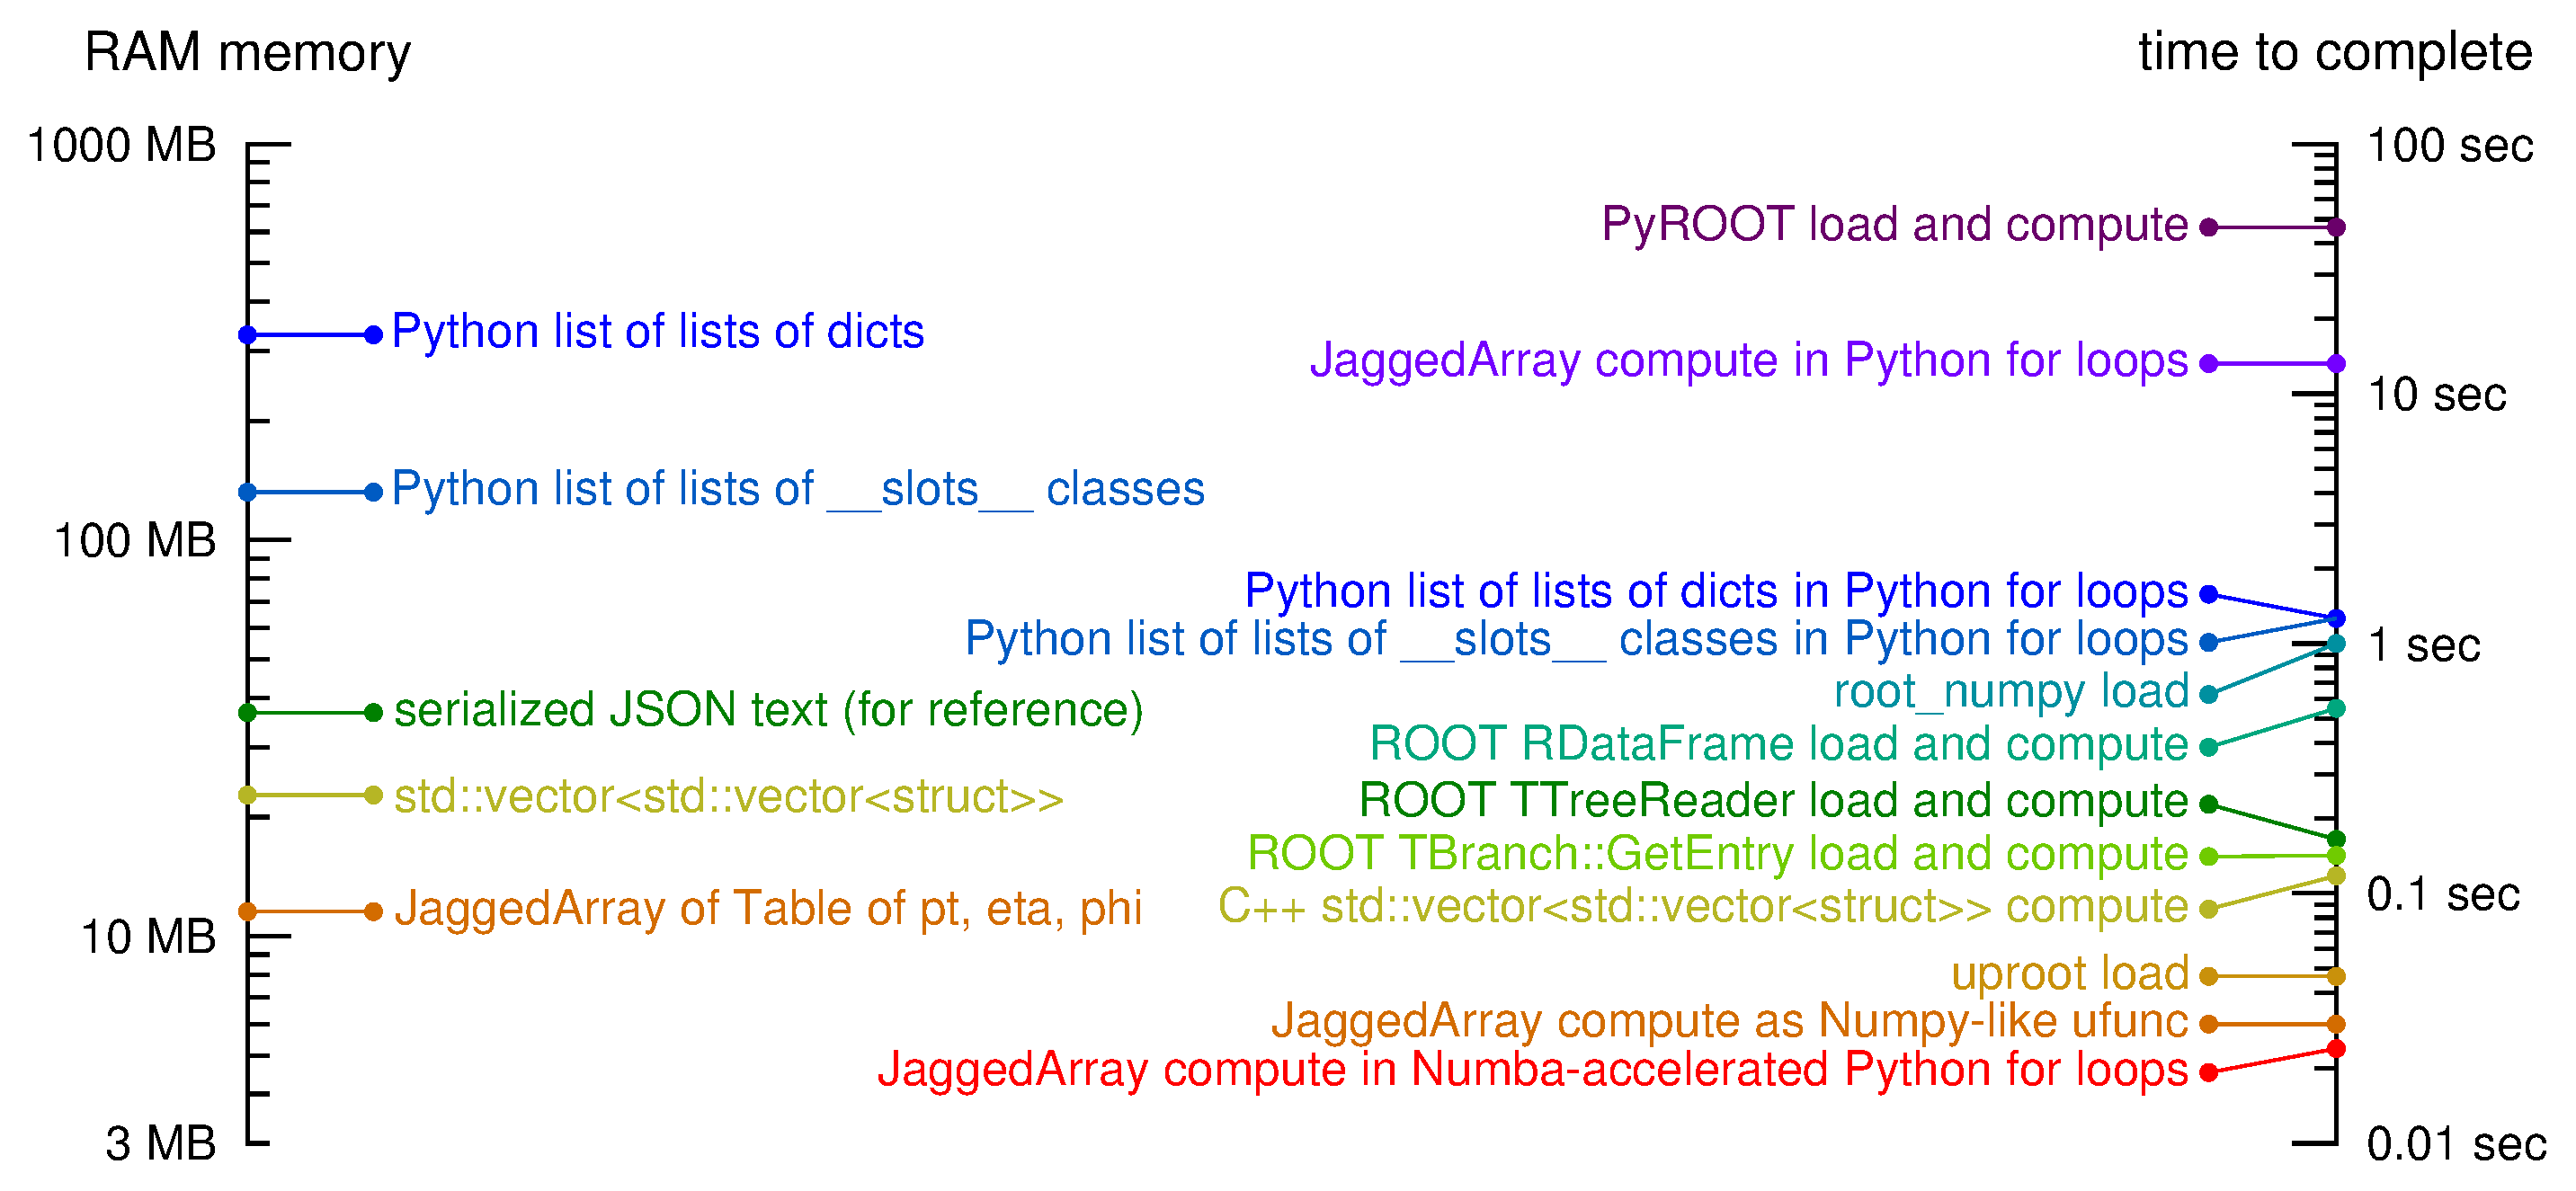
\includegraphics[width=\linewidth]{logscales.pdf}
\end{columns}
\end{frame}

\begin{frame}{Landscape of vertical performance}
\vspace{0.5 cm}
\scriptsize

\begin{columns}
\column{1.1\linewidth}
\begin{columns}
\column{0.38\linewidth}
\begin{tabular}{r p{0.9\linewidth}}
& \textcolor{darkblue}{\underline{RAM memory occupied by data (MB)}} \\
& \\
311.95 & \textcolor{pythoncolor}{Python list of lists of dicts} \\
215.11 & \textcolor{rootnpcolor}{root\_numpy's array of arrays} \\
139.79 & \textcolor{pythoncolor}{Python list of lists of {\tt\scriptsize \_\_slots\_\_} classes} \\
& \\
 37.19 & \textcolor{gray}{serialized JSON text (for reference)} \\
& \\
 22.38 & \textcolor{cppcolor}{\tt\scriptsize std::vector<std::vector<struct>>} \\
 11.67 & \textcolor{mycolor}{JaggedArray of Table of pt, eta, phi} \\
& \\
& \textcolor{gray}{\scriptsize 1 MB = 1024$^2$ bytes} \\
& \textcolor{gray}{\scriptsize 701,716 events containing 552,056 muons} \\
& \textcolor{gray}{\scriptsize storing pt, eta, phi as float32} \\
\end{tabular}

\vspace{2.3 cm}

\column{0.6\linewidth}
\begin{tabular}{r p{0.9\linewidth}}
& \textcolor{darkblue}{\underline{time to complete load, compute, or both (sec)}} \\
& \\
45.9\textcolor{white}{00} & \textcolor{rootcolor}{PyROOT load and compute} \\
12.9\textcolor{white}{00} & \textcolor{mycolor}{JaggedArray compute in Python for loops} \\
& \\
1.67\textcolor{white}{0} & \textcolor{rootnpcolor}{root\_numpy compute in loop over ufuncs} \\
 1.24\textcolor{white}{0} & \textcolor{pythoncolor}{Python list of lists of dicts in Python for loops} \\
 1.23\textcolor{white}{0} & \textcolor{pythoncolor}{Python list of lists of {\tt\scriptsize \_\_slots\_\_} classes in Python for loops} \\
& \\
 1.01\textcolor{white}{0} & \textcolor{rootnpcolor}{root\_numpy load} \\
& \\
 0.538 & \textcolor{rootcolor}{ROOT RDataFrame load and compute} \\
 0.164 & \textcolor{rootcolor}{ROOT TTreeReader load and compute} \\
 0.142 & \textcolor{rootcolor}{ROOT TBranch::GetEntry load and compute} \\
 0.113 & \textcolor{cppcolor}{{\tt\scriptsize std::vector<std::vector<struct>>} compute} \\
& \\
 0.047 & \textcolor{mycolor}{uproot load} \\
 0.030 & \textcolor{mycolor}{JaggedArray compute as Numpy-like ufunc} \\
 0.023 & \textcolor{mycolor}{JaggedArray compute in Numba-accelerated Python for loops} \\
& \\
& \textcolor{gray}{\scriptsize all with warmed disk cache} \\
\end{tabular}
\end{columns}
\end{columns}
\end{frame}

%% \begin{frame}
%% \huge
%% \begin{center}
%% \textcolor{darkblue}{Backup}
%% \end{center}
%% \end{frame}

%% \begin{frame}[fragile]{JaggedArray compute in Python for loops}
%% \vspace{0.3 cm}
%% \scriptsize
%% \begin{minted}{python}
%% %%timeit
%% k = 0
%% for event in events:
%%     for muon in event:
%%         pz[k] = muon.pt * math.sinh(muon.eta)
%%         k += 1
%% \end{minted}

%% \vspace{0.5 cm}
%% \hfill\begin{minipage}{0.6\linewidth}
%% {\normalsize \ldots with Numba acceleration:}
%% \begin{minted}{python}
%% import numba

%% @numpy.jit
%% def callme(pz, events):
%%     k = 0
%%     for event in events:
%%         for muon in event:
%%             pz[k] = muon.pt * math.sinh(muon.eta)
%%             k += 1

%% %%timeit
%% callme(pz, events)
%% \end{minted}
%% \end{minipage}
%% \end{frame}

%% \begin{frame}[fragile]{JaggedArray and root\_numpy ufuncs}
%% \scriptsize
%% {\normalsize JaggedArray compute as Numpy-like ufunc:}
%% \begin{minted}{python}
%% import numpy

%% %%timeit
%% pz = events["pt"] * numpy.sinh(events["eta"])
%% \end{minted}

%% \vspace{0.5 cm}
%% \hfill\begin{minipage}{0.6\linewidth}
%% {\normalsize root\_numpy compute in loop over ufuncs:}
%% \begin{minted}{python}
%% %%timeit
%% k = 0
%% for event in events:
%%     pt = event["Muon_pt"]
%%     eta = event["Muon_eta"]
%%     pz[k : k + len(pt)] = pt * numpy.sinh(eta)
%%     k += len(pt)
%% \end{minted}
%% \end{minipage}
%% \end{frame}

%% \begin{frame}[fragile]{Python list of lists of dicts/classes compute in Python for loops}
%% \scriptsize
%% \begin{columns}[t]
%% \column{0.5\linewidth}
%% \begin{minted}{python}
%% from math import sinh

%% events = [
%%     [],
%%     [{"pt": 129.8,
%%       "eta": -1.006,
%%       "phi": -0.581},
%%      {"pt": 73.08,
%%       "eta": -0.719,
%%       "phi": -1.51}],
%%     ...
%%     ]

%% %%timeit
%% k = 0
%% for event in events:
%%     for muon in event:
%%         pz[k] = (muon["pt"] *
%%                  sinh(muon["eta"]))
%%         k += 1
%% \end{minted}

%% \column{0.5\linewidth}
%% \begin{minted}{python}
%% class Muon(object):
%%     __slots__ = ["pt", "eta", "phi"]
%%     def __init__(self, pt, eta, phi):
%%         self.pt = pt
%%         self.eta = eta
%%         self.phi = phi

%% events = [
%%     [],
%%     [Muon(129.8, -1.006, -0.581),
%%      Muon(73.08, -0.719, -1.51)],
%%     ...
%%     ]

%% %%timeit
%% k = 0
%% for event in asobjs:
%%     for muon in event:
%%         pz[k] = (muon.pt *
%%                  sinh(muon.eta))
%%         k += 1
%% \end{minted}
%% \end{columns}
%% \end{frame}

%% \begin{frame}[fragile]{root\_numpy load and uproot load}
%% \scriptsize
%% \begin{minted}{python}
%% import ROOT
%% import root_numpy

%% file = ROOT.TFile("NanoAOD-DYJetsToLL.root")
%% tree = file.Get("tree")

%% %%timeit
%% root_numpy.tree2array(tree, ["Muon_pt", "Muon_eta", "Muon_phi"])




%% import uproot
%% tree = uproot.open("NanoAOD-DYJetsToLL.root")["tree"]

%% %%timeit
%% pt, eta, phi = tree.arrays(["Muon_pt", "Muon_eta", "Muon_phi"], outputtype=tuple)
%% \end{minted}
%% \end{frame}

%% \begin{frame}[fragile]{PyROOT load and compute}
%% \scriptsize
%% \begin{minted}{python}
%% import math
%% import numpy
%% import ROOT

%% file = ROOT.TFile("NanoAOD-DYJetsToLL.root")
%% tree = file.Get("tree")

%% tree.SetBranchStatus("*", 0)
%% tree.SetBranchStatus("nMuon", 1)
%% tree.SetBranchStatus("Muon_pt", 1)
%% tree.SetBranchStatus("Muon_eta", 1)

%% pz = numpy.empty(552056, dtype=numpy.float32)

%% %%timeit
%% k = 0
%% for event in tree:
%%     for pt, eta in zip(event.Muon_pt, event.Muon_eta):
%%         pz[k] = pt * math.sinh(eta)
%%         k += 1
%% \end{minted}
%% \end{frame}

%% \begin{frame}[fragile]{ROOT RDataFrame load and compute}
%% \vspace{0.1 cm}
%% \scriptsize
%% \begin{columns}
%% \column{1.05\linewidth}
%% \begin{minted}{c++}
%% #include <ctime>
%% #include <sys/time.h>
%% struct timeval starttime, endtime;

%% auto file = TFile::Open("NanoAOD-DYJetsToLL.root")
%% ROOT::RDataFrame rdf("tree", file);

%% TTree* tree; file->GetObject("tree", tree);   // perhaps unnecessary, but just in case...
%% tree->SetBranchStatus("*", 0);
%% tree->SetBranchStatus("nMuon", 1);
%% tree->SetBranchStatus("Muon_pt", 1);
%% tree->SetBranchStatus("Muon_eta", 1);

%% float pz[552056];
%% gettimeofday(&starttime, 0);
%% int k = 0;
%% rdf.Foreach([&k](ROOT::VecOps::RVec<float> Muon_pt, ROOT::VecOps::RVec<float> Muon_eta) {
%%     for (int i = 0;  i < Muon_pt.size();  i++) {
%%         pz[k]= Muon_pt[i] * sinh(Muon_eta[i]);
%%         k++;
%%     }
%% }, {"Muon_pt", "Muon_eta"});
%% gettimeofday(&endtime, 0);
%% \end{minted}
%% \end{columns}
%% \end{frame}

%% \begin{frame}[fragile]{ROOT TTreeReader load and compute}
%% \scriptsize
%% \begin{columns}
%% \column{1.05\linewidth}
%% \begin{minted}{c++}
%% #include <ctime>
%% #include <sys/time.h>
%% struct timeval starttime, endtime;

%% auto file = TFile::Open("NanoAOD-DYJetsToLL.root")
%% TTree* tree; file->GetObject("tree", tree);   // perhaps unnecessary, but just in case...
%% tree->SetBranchStatus("*", 0);
%% tree->SetBranchStatus("nMuon", 1);
%% tree->SetBranchStatus("Muon_pt", 1);
%% tree->SetBranchStatus("Muon_eta", 1);

%% TTreeReader reader("tree", file);
%% TTreeReaderArray<float> pt(reader, "Muon_pt");
%% TTreeReaderArray<float> eta(reader, "Muon_eta");

%% gettimeofday(&starttime, 0);
%% int k = 0;
%% while (reader.Next()) {
%%     for (int i = 0;  i < pt.GetSize();  i++) {
%%         pz[k] = pt[i] * sinh(eta[i]);
%%         k++;
%%     }
%% }
%% gettimeofday(&endtime, 0);
%% \end{minted}
%% \end{columns}
%% \end{frame}

%% \begin{frame}[fragile]{ROOT TBranch::GetEntry load and compute}
%% \vspace{0.2 cm}
%% \scriptsize
%% \begin{columns}
%% \column{1.1\linewidth}
%% \begin{minted}{c++}
%% #include <ctime>
%% #include <sys/time.h>
%% struct timeval starttime, endtime;

%% auto file = TFile::Open("NanoAOD-DYJetsToLL.root")
%% TTree* tree; file->GetObject("tree", tree);

%% UInt_t nMuon; float pts[10]; float etas[10];
%% TBranch* nbranch = tree->GetBranch("nMuon");       tree->SetBranchAddress("nMuon", &nMuon);
%% TBranch* ptbranch = tree->GetBranch("Muon_pt");    tree->SetBranchAddress("Muon_pt", pts);
%% TBranch* etabranch = tree->GetBranch("Muon_eta");  tree->SetBranchAddress("Muon_eta", etas);

%% gettimeofday(&starttime, 0);
%% int k = 0;
%% for (int i = 0;  i < 701716;  i++) {
%%     // TBranch::GetEntry, rather than TTree::GetEntry, avoids a loop over branches
%%     nbranch->GetEntry(i);    ptbranch->GetEntry(i);    etabranch->GetEntry(i);
%%     for (int j = 0;  j < nMuon;  j++) {
%%         pz[k] = pts[j] * sinh(etas[j]);
%%         k++;
%%     }
%% }
%% gettimeofday(&endtime, 0);
%% \end{minted}
%% \end{columns}
%% \end{frame}

%% \begin{frame}[fragile]{{\tt std::vector<std::vector<struct>>}}
%% \vspace{0.3 cm}
%% \scriptsize
%% \begin{minted}{c++}
%% struct Muon {
%%     float pt;
%%     float eta;
%%     float phi;
%% };

%% struct Event {
%%     std::vector<Muon> muons;
%% };

%% auto events = // std::vector<std::vector<Muon>>, filled with push_back

%% gettimeofday(&starttime, 0);
%% int k = 0;
%% for (int i = 0;  i < events.size();  i++) {
%%     for (int j = 0;  j < events[i].muons.size();  j++) {
%%         pz[k] = events[i].muons[j].pt * sinh(events[i].muons[j].eta);
%%         k++;
%%     }
%% }
%% gettimeofday(&endtime, 0);
%% \end{minted}
%% \end{frame}

\end{document}
